\documentclass[12pt,letterpaper]{article}
\usepackage{fullpage}
\usepackage[top=2cm, bottom=4cm, left=2cm, right=2cm]{geometry}
\usepackage{amsmath,amsthm,amsfonts,amssymb,amscd}
\usepackage{lastpage}
\usepackage{enumerate}
\usepackage{fancyhdr}
\usepackage{mathrsfs}
\usepackage{xcolor}
\usepackage{graphicx}
\usepackage{listings}
\usepackage{hyperref}
\usepackage{siunitx}
\usepackage{appendix}
\usepackage{caption}
\usepackage{subcaption}
\usepackage{multicol}
\usepackage{wrapfig}

\hypersetup{%
  colorlinks=true,
  linkcolor=blue,
  linkbordercolor={0 0 1}
}
 
\renewcommand\lstlistingname{Algorithm}
\renewcommand\lstlistlistingname{Algorithms}
\def\lstlistingautorefname{Alg.}

\lstdefinestyle{Python}{
    language        = Python,
    frame           = lines, 
    basicstyle      = \footnotesize,
    keywordstyle    = \color{blue},
    stringstyle     = \color{green},
    commentstyle    = \color{orange}\ttfamily
}

\setlength{\parindent}{0.0in}
\setlength{\parskip}{0.05in}

% Edit these as appropriate
\newcommand\course{ASTRO 732}
\newcommand\coursename{Computational Methods for Physics}
\newcommand\hwnumber{2}                  % <-- homework number
\newcommand\myname{Sandra Bustamante}           % <-- NetID of person #1

\pagestyle{fancyplain}
\headheight 35pt
\lhead{\course \\ Homework \hwnumber}
\chead{\textbf{\Large The Golfer and the Monkey}}
\rhead{\myname \\ September 20, 2019}
\lfoot{}
\cfoot{\coursename}
\rfoot{\small\thepage}
\headsep 1.5em

%%%%%%%%%%%%%%%%%%%%%%%%%%%%%%%%%%%%%%%%%%%%%%%%%%%%%%%%%%%%%%%
%=====================BEGIN DOCUMENT===========================
%%%%%%%%%%%%%%%%%%%%%%%%%%%%%%%%%%%%%%%%%%%%%%%%%%%%%%%%%%%%%%%
\title{The Golfer and the Monkey}

\begin{document}
%\twocolumn

\begin{quote}
    \textit{A monkey has been stealing your bananas everyday for a month now. You are thinking what can you do to resolve this problem on your way to golf practice. Suddenly, you see something moving on a tree. It's HIM. On closer inspection, he looks like he is waiting for you to leave your house and steal your fresh bananas. 'No way!' you think and decide to scare the monkey away from your fruit. You prepare to shoot at him your golf ball. You estimate he is at about \SI{2000}{\m} away at a height of, probably, \SI{60}{\m}. What angle will you shoot?}
\end{quote}

%=========PROBLEM 1============================================
\section*{Background}
This game revisits the classic problem of the Hunter and the Monkey. The monkey is at a distance away from the hunter. The hunter aims at the monkey at some angle and at the time he shoots, the monkey falls down from a tree. The question is at what angles will it result in a hit.

The solution to this problem can be solved analytically by utilizing the equations of motions derived from Newton's Law:
\begin{align}
    \vec{x} &= \vec{x}_0 + \Vec{v}_0*t + \frac{1}{2} \vec{a}*t^2 \\
    \vec{v} &= \vec{v}_0 + \vec{a}*t
\end{align}

Another approach is utilizing the differential form of Newton's Law, 
\begin{equation}
    \vec{F}=m\Ddot{a}
\end{equation}
and solving it numerically with the fourth order Runge-Kutta method. 

The Runge-Kutta method can be described as calculating the slope on a point an advancing a step of size $h$. Then use the previous result to calculate the slope at half step. Then, repeat but now using the last result. Then again, use the last result to calculate the slope but now advance a whole step. Finally, use the information from all the steps to calculate your next value. This process is visually explained on Figure \ref{fig:rk4Example}. Computationally, we need to program the following equation:

\begin{figure}[ht]
    \centering
    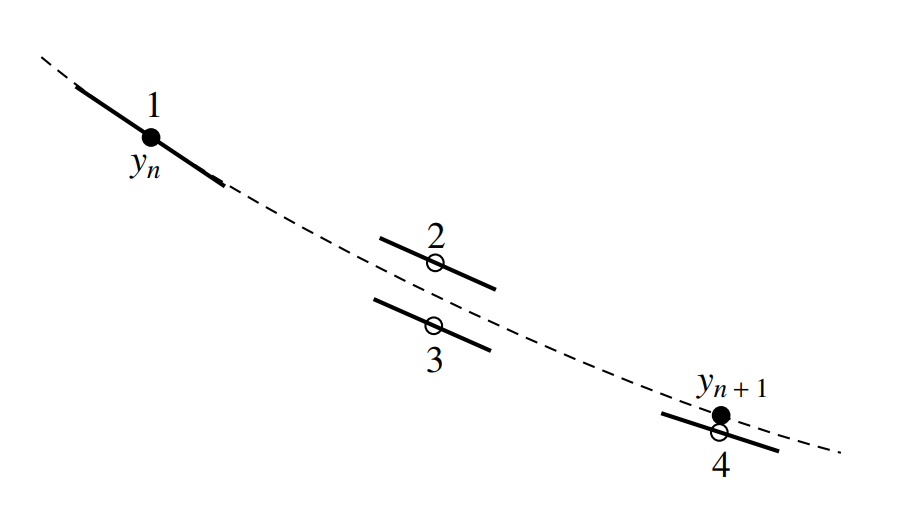
\includegraphics{rk4Example.png}
    \caption{Visually explain the fourth order Runge-Kutta method. \small{Source: Numerical Recipes 3rd Ed pg. 909}}
    \label{fig:rk4Example}
\end{figure}

\begin{align*}
    k_1 &= hf(x_n, y_n)\\
    k_2 &= hf(x_n + \frac{1}{2}h, y_n + \frac{1}{2}k_1)\\
    k_3 &= hf(x_n + \frac{1}{2}h, y_n + \frac{1}{2}k_2)\\
    k_4 &= hf(x_n + h,y_n + k_3)\\
    y_{n=1} &= y_n + \frac{1}{6}k_1 + \frac{1}{3}k_2 + \frac{1}{3}k_3 + \frac{1}{6}k_4
\end{align*}

Another approach

This differential equation can be solve by using Runge-Kutta. 


This game is comprised of 3 different play modes:

\begin{itemize}
    \item Easy: The only force acting on the bullet is the gravity.
    \item Medium: The forces acting on the bullet are gravity and air drag
    \item Difficult: The forces acting on the bullet are gravity, air resistance and a random wind.
\end{itemize}

Initial Conditions:
\begin{itemize}
    \item Horizontal distance between golfer and monkey is \SI{2000\pm 100}{\m}
    \item Vertical distance \SI{60 \pm 20}{\m}
    \item Approximate an spherical bullet with radius \SI{7.2}{\mm}
    \item Bullet mass of \SI{0.007}{\kilo\gram}
    \item Initial bullet velocity is \SI{1100}{\m\per\sec}
    \item Monkey's hit area is a circle with radius of \SI{10}{\mm}
\end{itemize}

\section*{Part 1: Easy Mode}

%=========PROBLEM 2============================================
\section*{Problem 2}

The AzTEC mm-wavelength camera completed a large survey of the COSMOS field in search for sub-millimeter galaxies. 
A typical source detection is between 4 and 10 sigma level. 
Before analyzing the data, is important to understand the noise properties of the camera. 
To do this, noise maps are produced. A noise map is a map with little to no astronomical signal. 
In this problem, a noise map of AzTEC was given. We need to produce two histograms, one linear and another in semi-log form, of the data within the center 20 arc-minutes of the map. 
The pixel size is $3 \times 3$ arc-seconds.

The steps followed to do the histograms are the following:

\begin{enumerate}
    \item Import fits file and read header.
    
    FITS stands for Flexible Image Transport System. It is a standard used mainly in astronomy to save data of the observations in a standard way. To import a fits file into Python so that the data can be accessed, a viewer is needed. It was recommended to use PyFits which was ported to Astropy as "astropy.io.fits". For this reason, astropy was used for this and subsequent problems as needed. 
    
    Once the fits viewer was imported, 
    \lstinline[columns=fixed, style=Python]{fits.open()} 
    will open the fits file. The fits file is compose of a list of objects which are compose of two parts: a header and the data. The header is were the metadata of the image is located. It gives information such as the timestamp, the instrument used, the number of axes, the number of pixels, etc. These parameters can be put into a variable by calling them by their label. 
    
    \item Extract the data of the centered 20 arcminutes.
    
    A mask is used to achieve this step. A mask is a matrix of the same size as the data which contains boolean values. If True, the data will stay as is and if False, the data will be turn into zero. This process will only "make visible" the data we are interested. 
    
    The mask "shape" will be a circle since the information needed is the within 20 arcminutes of the center of the map. Using the header, the location of the central pixel can be estimated by taking the length of the axis and divide it by 2. It is known that the equation of the circle is given by 
    \begin{equation} \label{eq:circle}
        r = \sqrt{(x-x_0)^2 + (y-y_0)^2}
    \end{equation}
    where $x_0$ and $y_0$ are the coordinates of the center and $r$ is the radius of the circle. 
    
    The radius of the circle is 20 arcminutes which transformed into pixels, given that each pixel is 3 arcseconds, is 
    \begin{equation}\label{eq:radiusInPixels}
        r= 20' \times \frac{60''}{1'} \times \frac{1  \mathrm{pixel}}{3''} = 400 \mathrm{pixel}
    \end{equation}
    
    Comparing the right hand of equation \ref{eq:circle} bigger than r in pixels, outputs a boolean array with same dimensions as the data, in other words, it creates the mask. The mask is applied to the data and later trimmed so it will contain the information wanted. 
    
    \item Create histograms.
    
    An histogram shows how many times the values in a range are repeated. The range is given by the bin size. Since the values are being counted, the positions of the values are not important at this point. The \lstinline[columns=fixed, style=Python]{data.flatten()} command makes the 2 dimensional array into a 1 dimensional array. After this, the data is ready to get the histogram. 
    
    The histograms of the values are given by Figure \ref{fig:histograms}. 
    
    \begin{figure}[]
        \centering
        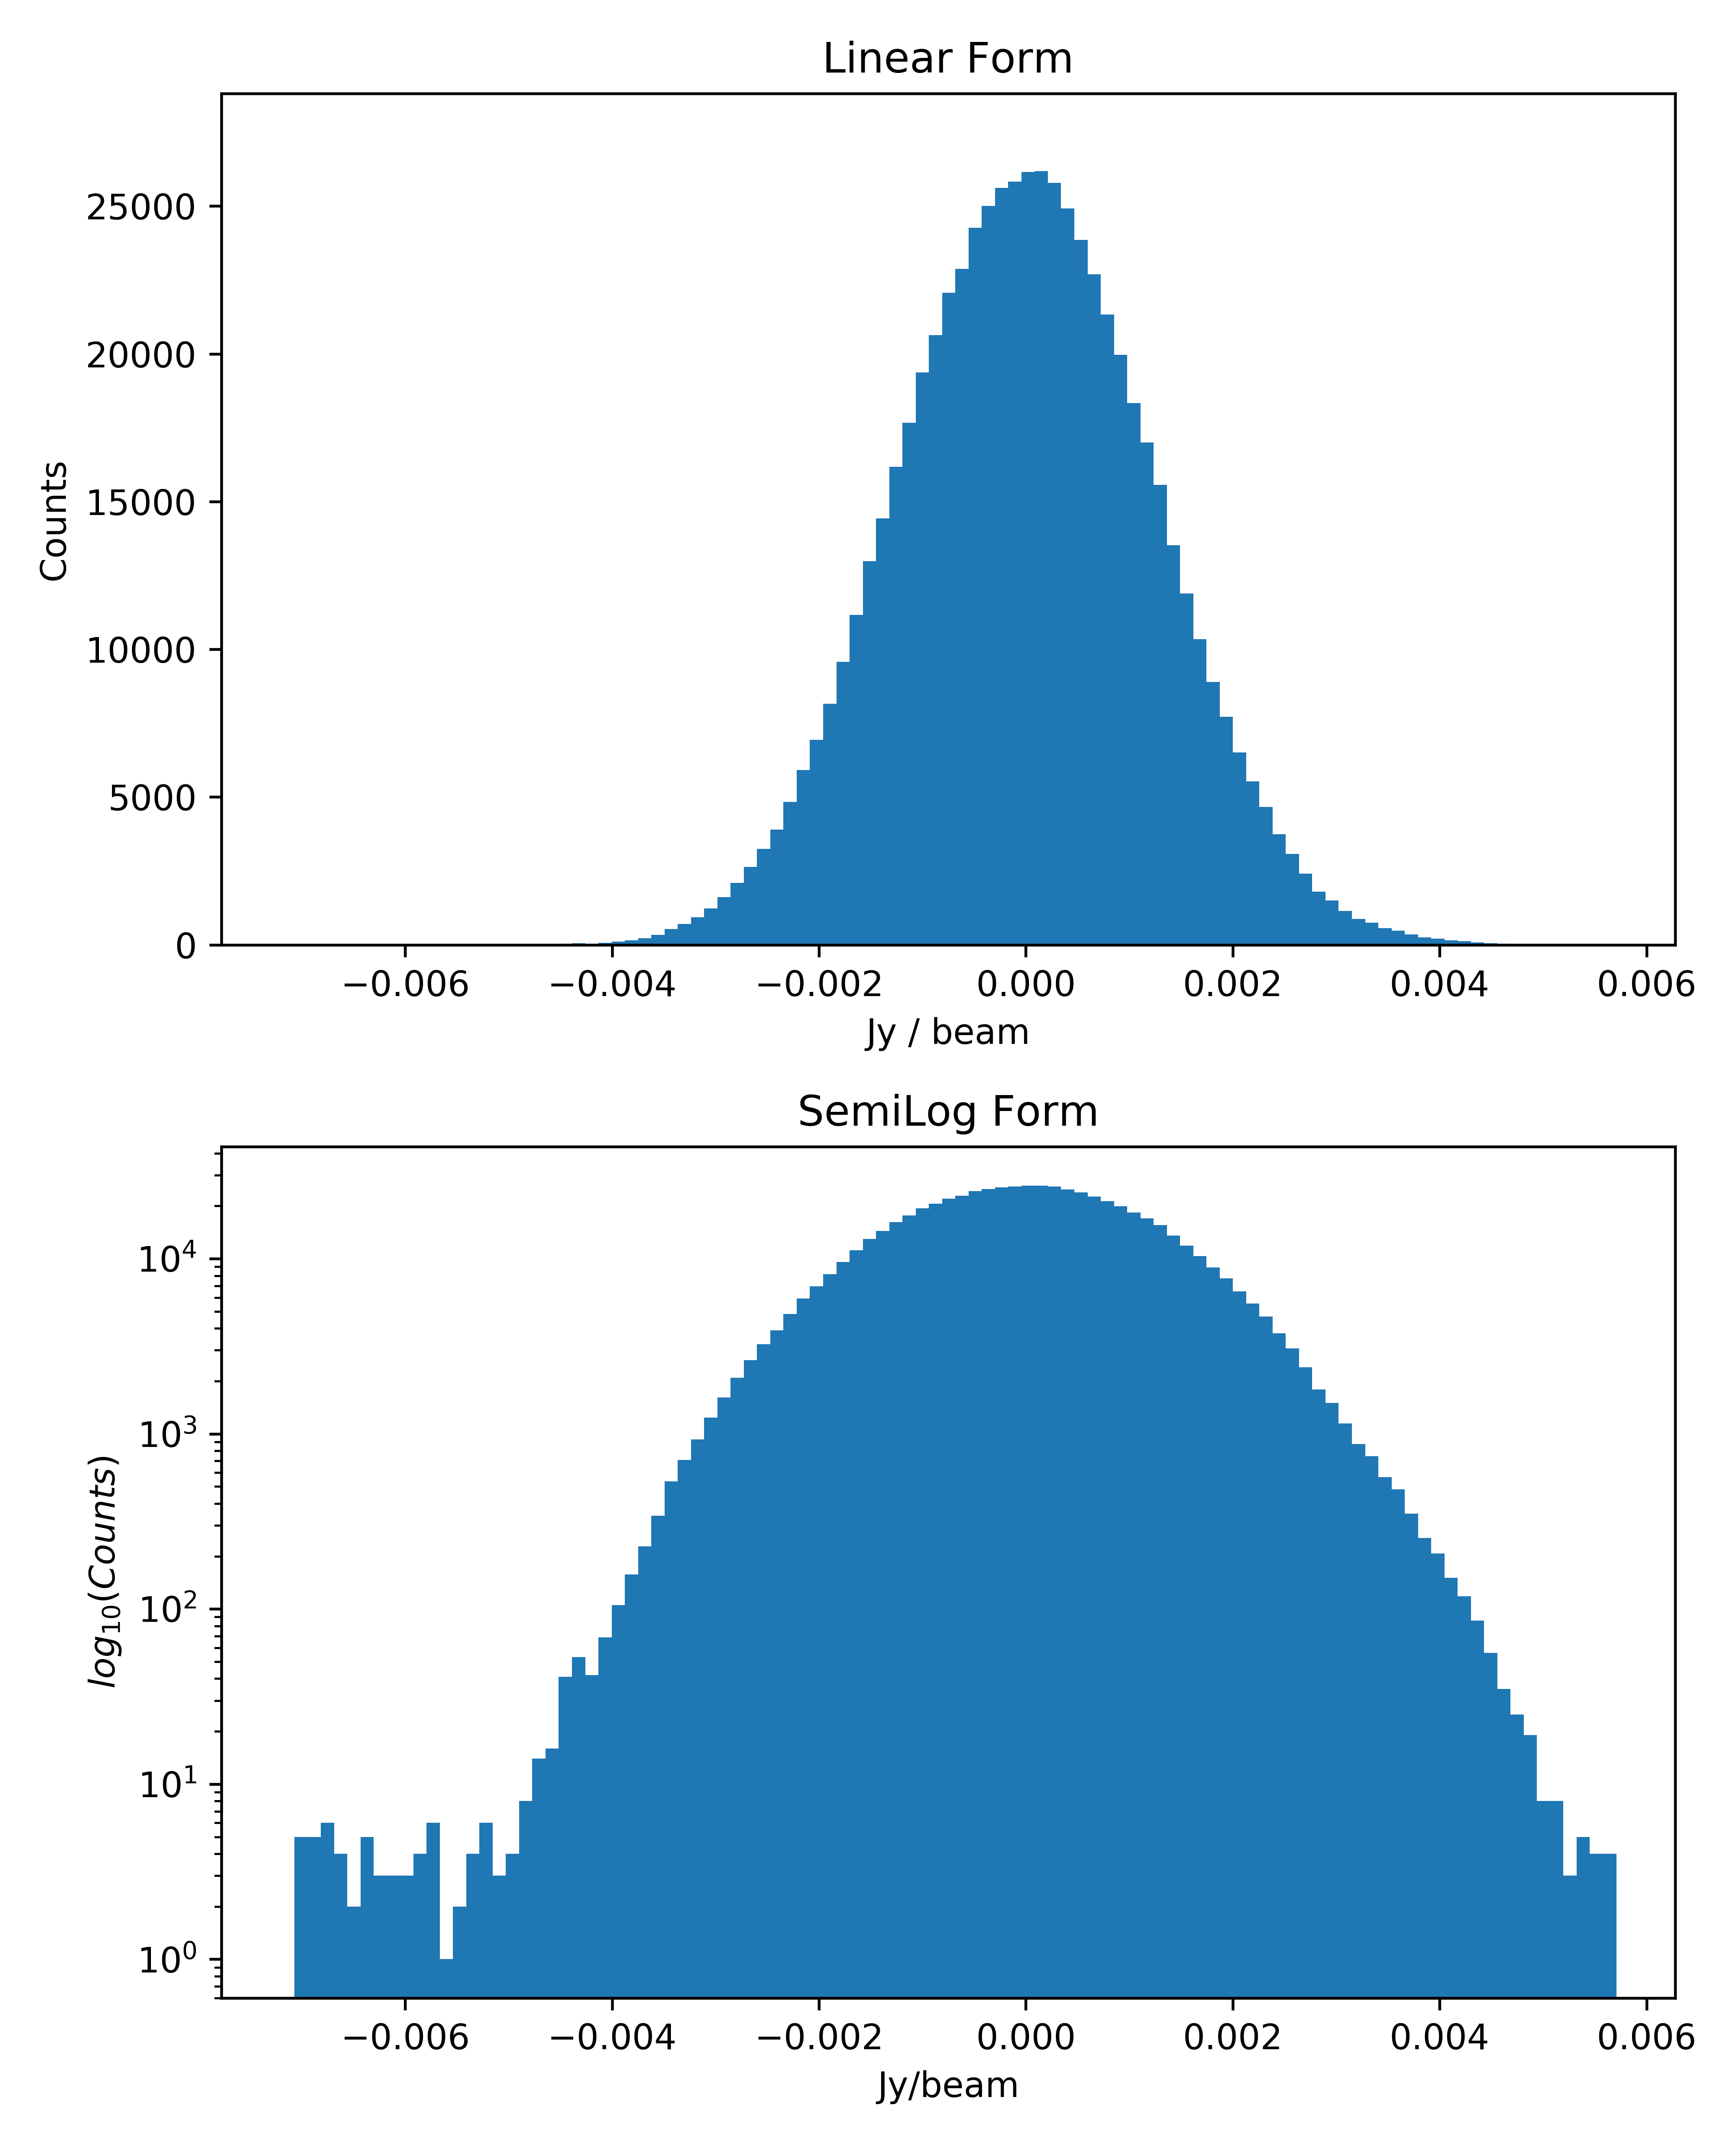
\includegraphics{figures/hw01prob1-2fig1.png}
        \caption{Histograms of the noise map of AzTEC. Top: Histogram in a linear form. Bottom: Histogram in a semi-log form.}
        \label{fig:histograms}
    \end{figure}
    
     \item \textbf{Customize the plot to achieve a readable and understandable plot.}
     
\end{enumerate}

The histogram in its linear form shows a bell-like shape. This shape is associated to a normal distribution or to a Gaussian. The mean of the data will be the center of this shape. This suggests that the noise is produced by a random process.

The histogram in its semilog form shows a more rounded shape.This shows that most values are near the center. 

%=========PROBLEM 3============================================
\section*{Problem 3}

The AzTEC mm-wavelength camera completed a large survey of the COSMOS field in search for sub-millimeter galaxies. 
A typical source detection is between 4 and 10 sigma level. 

In this problem, the data composed of the signal to noise ratio is given. We need to produce an image of the data within 20 arc-minutes. In addition, we need to identify the source candidates with signal to noise ratio grater than 4.5.
The pixel size is $3 \times 3$ arc-seconds.

The steps followed to do the image are very similar to Problem 2:

\begin{enumerate}
    \item Import fit file and read header.
    
    Same as before
    
    \item Extract sky coordinates.
    
    As mentioned previously, the header contains metadata of the image including the coordinates in pixels of a reference pixel and its corresponding coordinates in the sky. All of these information, among others, is used to create a "projection" of the pixels into sky coordinates which is later use when plotting the data.
    
    \item Extract the data of the centered 20 arcminutes.
    
    Same as before.
    
    \item Create image of signal to noise ratio with a color bar.
    
    During initialization of the figure is necessary to include the command \lstinline[columns=fixed, style=Python]{projection=wcs}. This command will allow that the plot will show on world coordinates instead of pixel coordinates. It also allows that future x and y values can be given in both coordinate systems. 
    
    The command \lstinline[columns=fixed, style=Python]{imshow()} is used. Since the pixel is $3 \times 3$, it means is square so \lstinline[columns=fixed, style=Python]{aspect='equal'} is used so that the x and y axis have the same size. 
    
    \item Add circles to source candidates.
    
    To do this, is necessary to first determine the coordinates of such sources. The command \lstinline[columns=fixed, style=Python]{np.where(data>4.5)} returns the values of the pixels that satisfy the inequality. This x and y values are use in a scatter plot with the property facecolor='none'. Consequently, circles are plotted on source candidates. 
    
    Improvements needed: For sources that extend to more than one pixel, the center coordinate needs to determined so instead of having several circle squish together, it'll show a single circle around the source candidates. 
    
    \item Customize plot
    
\end{enumerate}

The image of the signal to noise ratio is shown on Figure \ref{fig:image}.

 \begin{figure}[h]
        \centering
        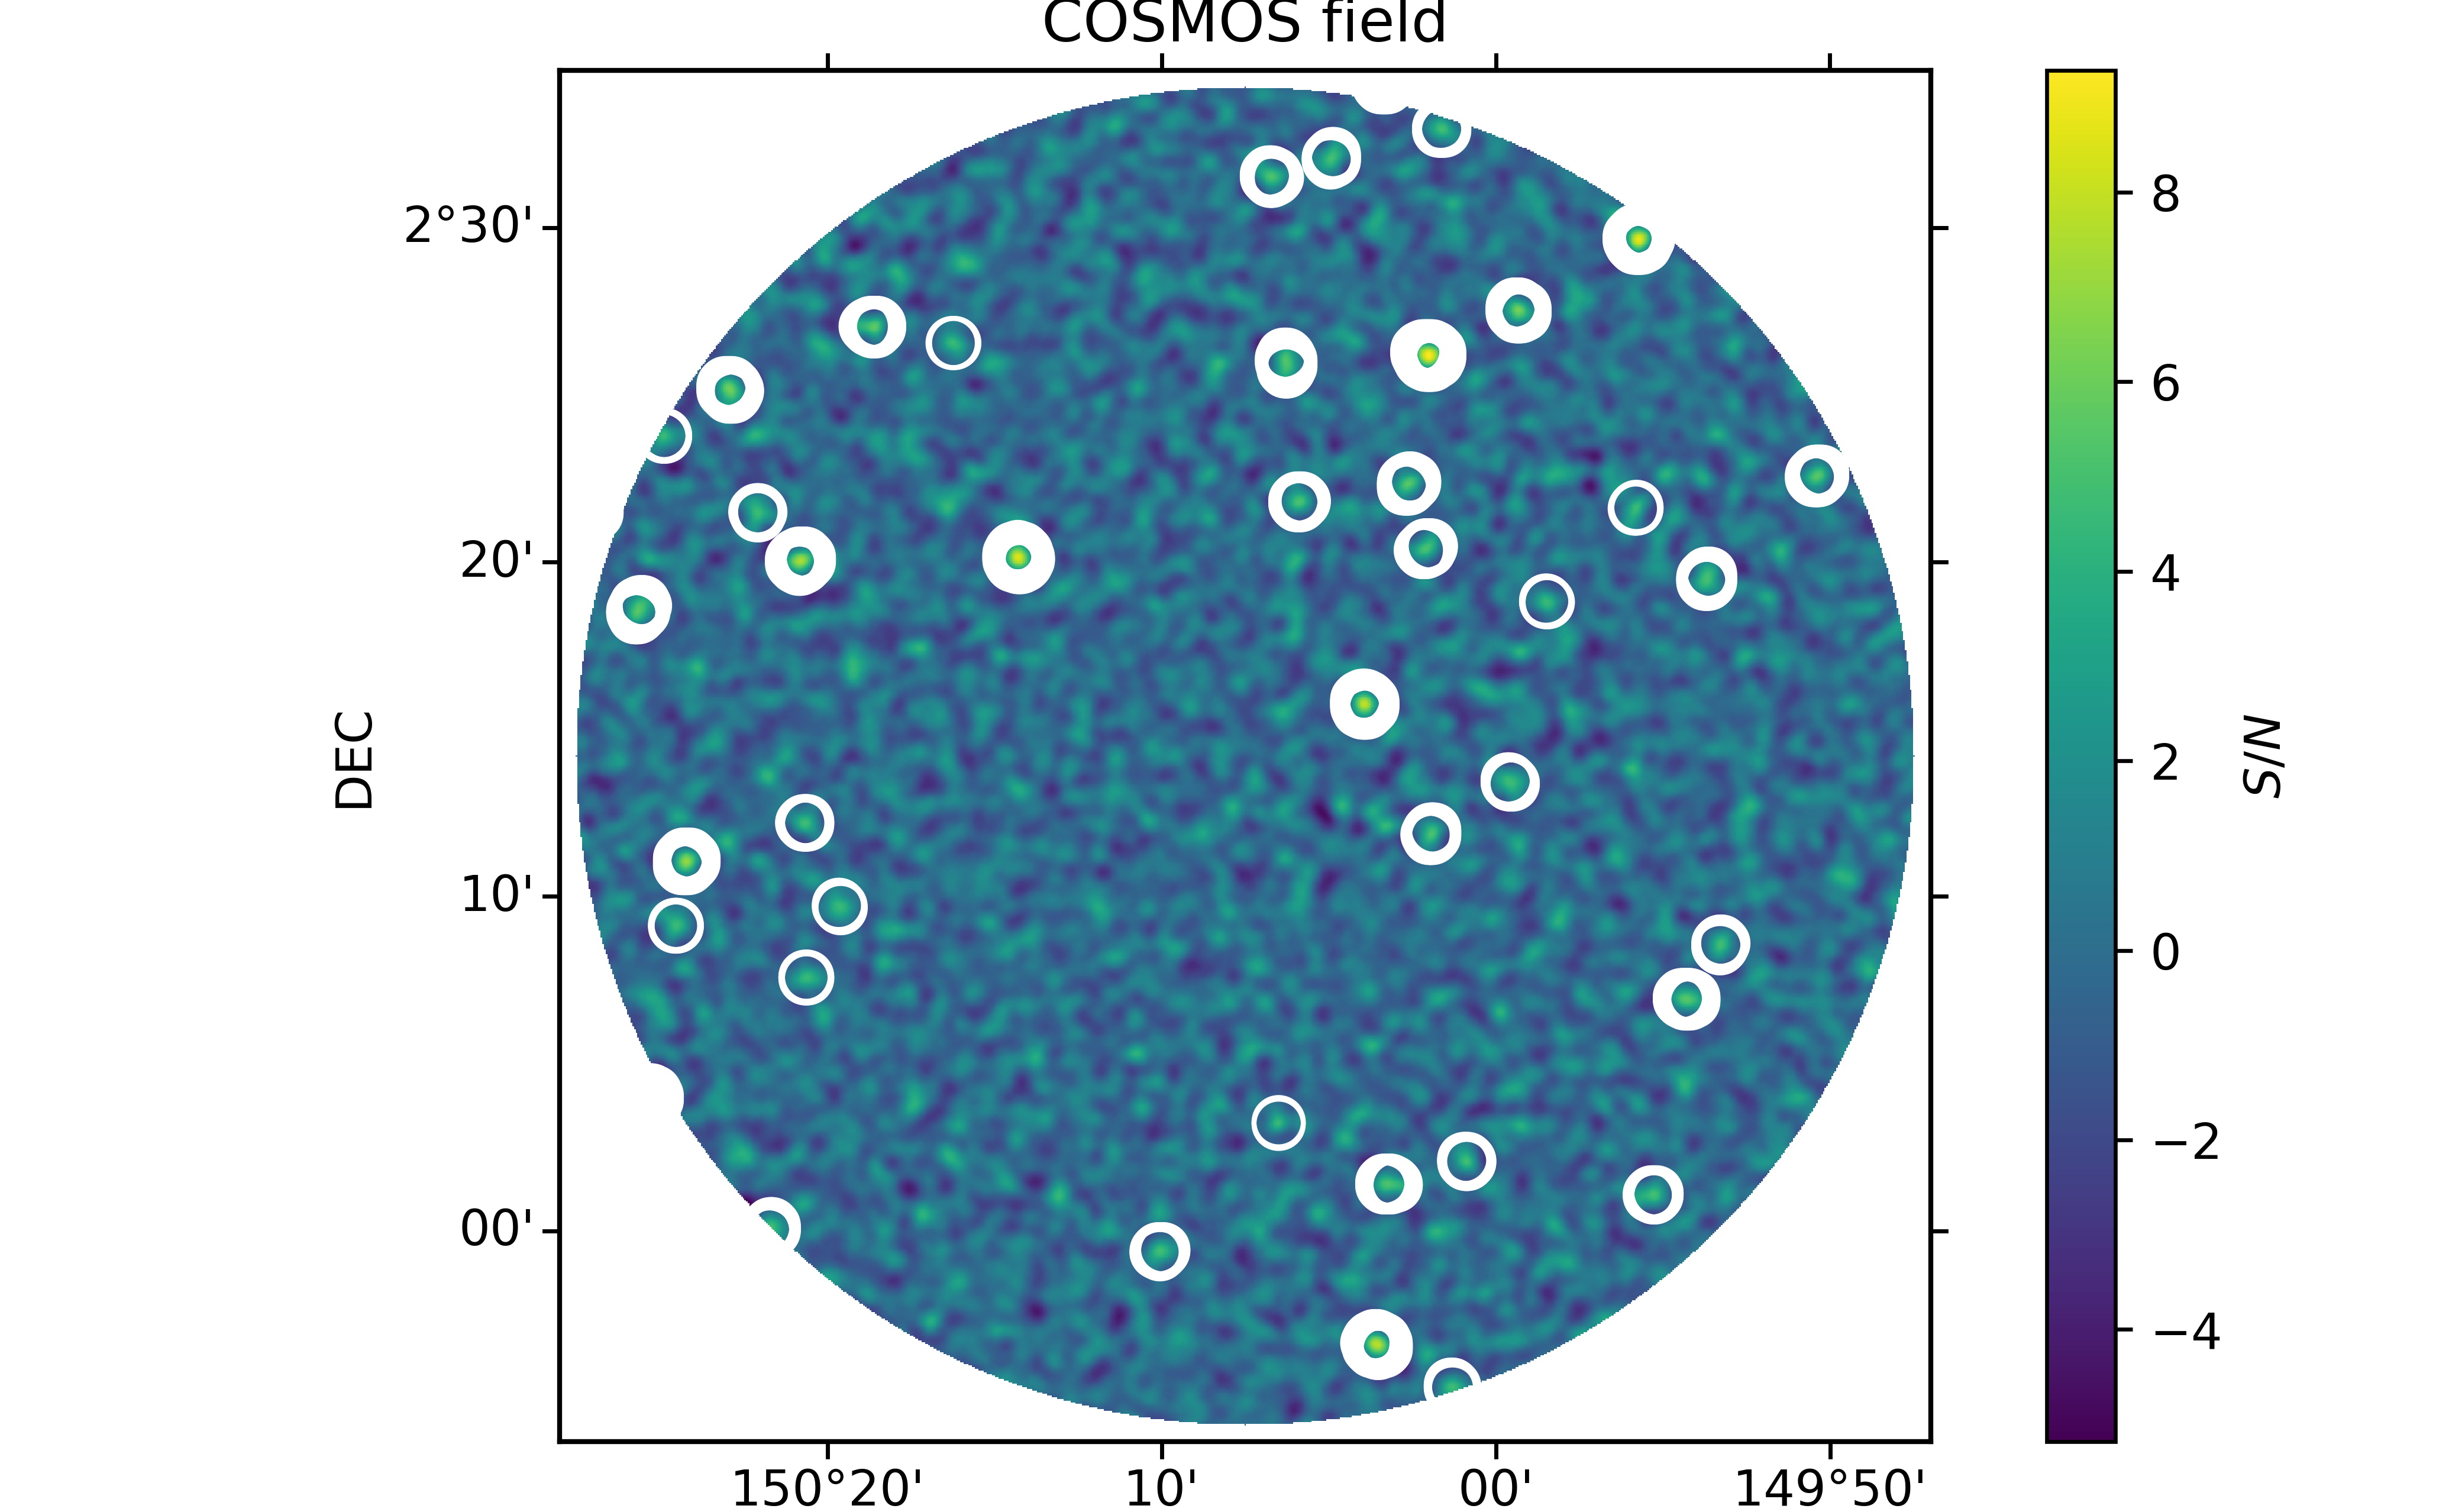
\includegraphics{figures/hw01prob1-3fig1.png}
        \caption{Signal to Noise Ratio of COSMOS field using AzTEC.}
        \label{fig:image}
    \end{figure}


%     
%\include{name} %name without extension. insert in new page

\newpage
\appendix

\lstset{caption={hw02.py}, style=Python}

\section[]{Python code to solve Homework 2} 
\label{sec:CodeHw02}
\lstset{label={hw02.py}}
\lstinputlisting[language=Python]{hw02.py}


% \newpage
% \section[]{Python Code to Solve Problem 5} 
% \label{sec:CodeHw01-5}
% \lstset{label={hw01prob1-5.py}}
% \lstinputlisting[language=Python]{code/hw01prob1-5.py}

\end{document}